% find this class at https://archive.danleonard.us/scholarship/coursework/coursework.cls
\documentclass{../../../coursework}

\title{Indigenization in Magna Graecia:}
\subtitle{The Case of Sicily}
\shorttitle{Indigenization in Magna Graecian Sicily}
\author{Daniel}{Glenn}{Leonard}
\newdate{date}{3}{5}{2019}
\date{\displaydate{date}}
\course{CLCV}{444}{The Archaeology of Italy}{University of Illinois at Urbana-Champaign}
\instructor{Dr}{Brett}{Sanford}{}{Kaufman}

\keywords{}
\addbibresource{sicily.bib}
%\addbibresource[location=remote]{https://archive.danleonard.us/scholarship/coursework/illinois/CLCV/444/sicily.bib}
\baseurl{https://archive.danleonard.us/scholarship/coursework/illinois/CLCV/444/sicily.xhtml}

\begin{document}

\maketitle

\section{Introduction}

Sicily's geographic position in the Mediterranean Sea allowed it to be
conferred strategic advantages by several generations of Classical-era
empires. Phoenicians, Greeks, and Romans all at some point colonized the
island of Sicily for trade, material wealth, and military advantage. At the
same time, indigenous Sicilian societies reckoned with the encroachment of
foreign empires upon their island. This interrelation between indigenous and
imperial played out in a variety of ways in ancient Sicily, creating a
microcosm of Classical-era empire and conquest.

\section{History of Sicilian Colonization}

\subsection{Indigenous Sicilian Context}

\begin{figure}
    \centering
    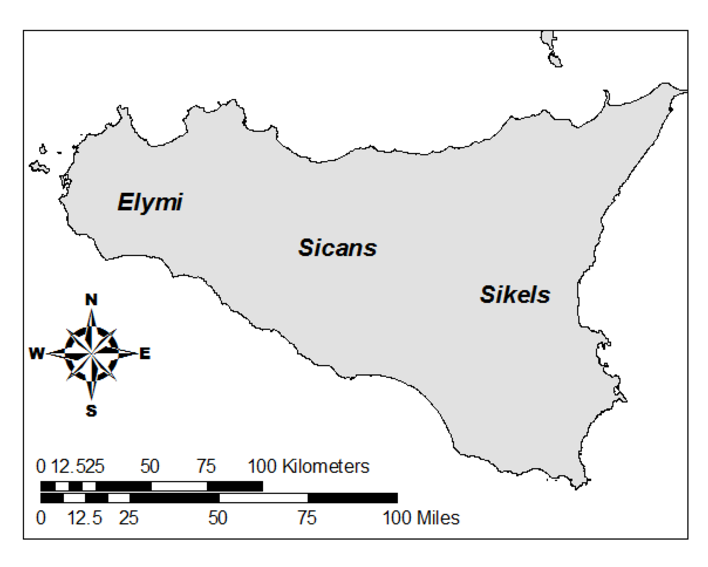
\includegraphics[width=0.7\textwidth]{sicily_fig_balco.eps}
    \caption{Map showing the general distribution of Iron Age Sicilian
    cultures based on ancient texts. Reprinted from \fullcite{Bal12}.
    Copyright \citeyear{Bal12} by \citeauthor{Bal12}}
    \label{fig:Balco}
\end{figure}

The vast majority of our understanding of indigenous Sicilians comes from the
Greek general \citeauthor{Thucydides}, whose History of the Peloponnesian War
devotes much of its sixth book to the history and current affairs of Sicilian
colonies. \citeauthor{Thucydides} describes three independent societies living
within Sicily at the time of Greek colonization, namely Elymi, Sicani, and
Sicels (for a map of the locations given by historical writers, see
Figure~\ref{fig:Balco}). The Greeks believed Sicily to have been the home of
Cyclopes and Laestrygonians, thus considering the three ethnic groups
encountered to have been recent immigrants who displaced the creatures of
legend \parencite[VI.2]{Thucydides}. Modern scholars have however attributed
these ethnic groups to inhabitation since at least 1270 BCE \parencite{Lei99}.

\citeauthor{Thucydides} described the Sicani as Iberian settlers who initially
displaced the mythical beasts of Sicily \parencite[VI.2]{Thucydides}. However,
modern scholarship opposes this origin. While scholars today agree with
\citeauthor{Thucydides} that the Sicani had the longest history of Sicilian
inhabitation at the time of Greek conquest, there is evidence for their
descent from the Illyrian peoples of the Balkans \parencite{Fin83}.
Culturally, historians have described a historical Sicani claim to have
``sprung from the earth'' in Sicily \parencite[12]{Fre92}, evidence of the
people's internal myth of indigeneity.

On the Western portion of the island lay the Elymians, whose social structure
revolved around the two large cities of Segesta and Eryx
\parencite[VI.2]{Thucydides}. The Greeks attributed their origin to the
inhabitants of Troy, a view that would persist into Roman times
\parencite{Fre92}. There is no known evidence to suggest a Trojan origin,
although it is possible that the Elymi descend from seafaring peoples in Asia
Minor. Their language remains undeciphered, yet it has been asserted that it
is likely Indo-European \parencite{Mar12} in contrast to the language isolate
of the Sicani.

Finally, the Sicels inhabited the eastern portion of the island. At the time
of Greek colonization, this group displayed bronzeworking skill and spoke a
decidedly Indo-European language.

\begin{figure}
    \centering
    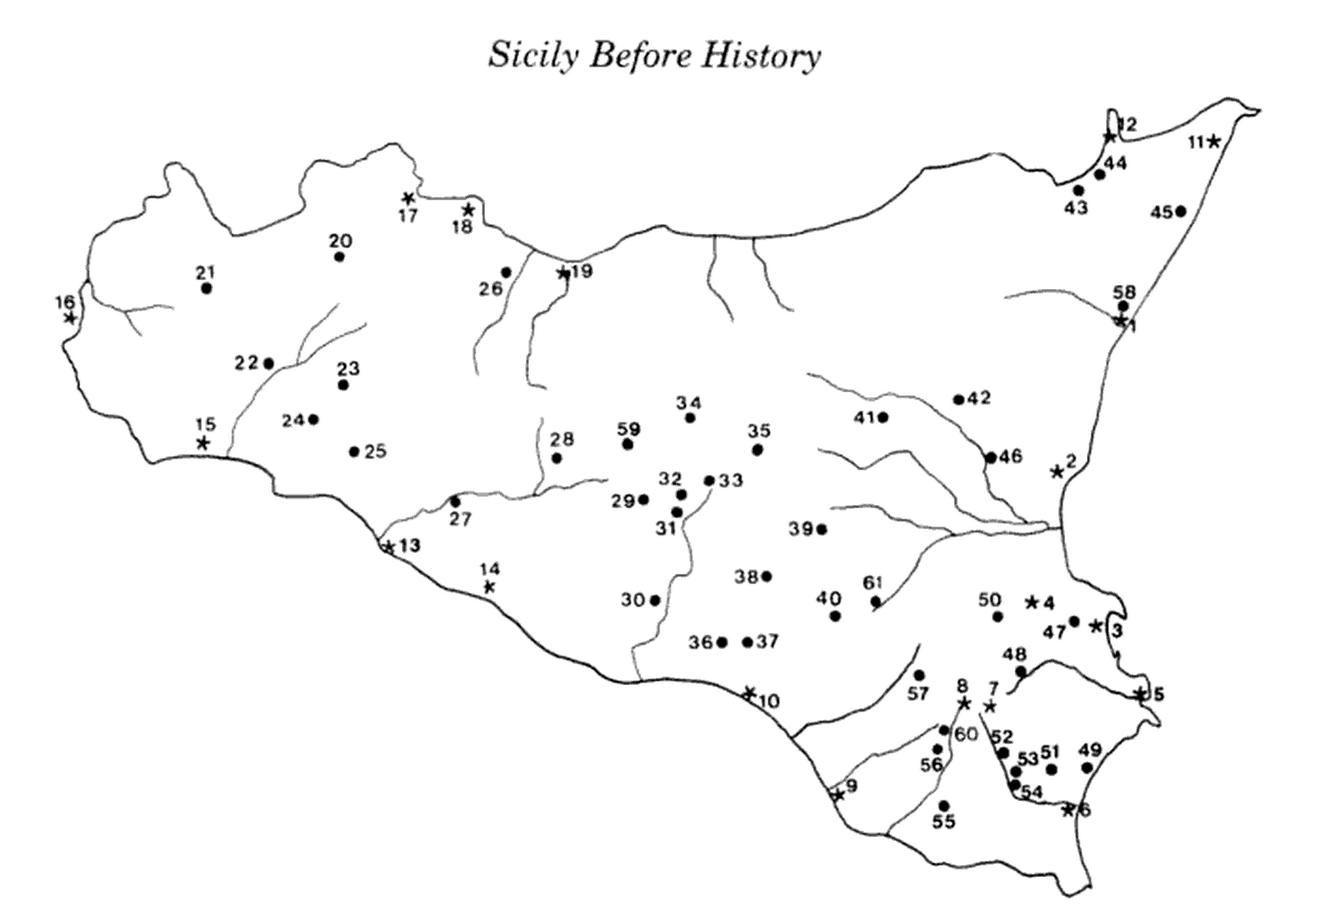
\includegraphics[width=0.75\textwidth]{sicily_fig_leighton.png}
    \caption{Map of archaeological sites in Sicily. Dots represent indigenous
    sites, stars represent Greek and Phoenician sites. Reprinted from
    \fullcite[222]{Lei99}. Copyright \citeyear{Lei99} by \citeauthor{Lei99}}
    \label{fig:Leighton}
\end{figure}

Despite these seemingly clear and named divisions of Sicily's precolonial
peoples, it has been recently called into question whether such distinct
cultures can be identified archaeologically. \textcite{Lei99} points out that
there has been difficulty in outlining three independent material cultures,
despite avid archaeological work on this island. In fact, the vast majority of
known archaeological sites on Sicily are of indigenous communities (see
Figure~\ref{fig:Leighton}). Likewise, \textcite{Bal12} notes that many of the
Greek histories of these three cultures differ greatly, often contradicting
one another.

\subsection{Early Colonization}

\subsubsection{Geographic Location}

Sicily is located in the center of the Mediterranean Sea, providing many
advantages for colonizing empires. Its highly diverse soils \parencite{Bal68}
are exceptionally fertile, allowing for the production of olives, grapes, and
grains, assets that have been vital to Mediterranean civilizations for
millennia \parencite{Bal12}. The location relative to the European and North
African mainlands provides further advantages, in control of
inter-Mediterranean trade, a fact that did not go unnoticed by Greeks or
Phoenicians \parencite{DeA03}.

\subsubsection{Phoenician Settlement}

Phoenicians have long been credited with early settlement of Sicily:
\citeauthor{Thucydides} gives a date of at least the 10th century BCE, and
historians had frequently used that date for the first founding of Phoenician
colonies. However, there is little to no archaeological evidence to support
such an assertion. The first sign of any Phoenician settlement is the presence
of imported Greek pottery on the western offshore island of Motya, which dates
only to 720 BCE \parencite{Lei99}. Carthaginians rapidly formed settlements on
several islands off the coasts of Sicily, as was common practice for
Phoenician settlement. However, \textcite{Fre92} notes that only in the
western cape were such settlements large enough as to be considered colonies,
with claimed territory attached to the city proper. Motya specifically would
grow to wield great influence in the region, benefitting from its location on
a small island in a sheltered and easily-defended bay. In addition Phoenicians
built cities inland, such as Solous and Panormos in a northern bay, which
allowed for large volumes of trade with much of Europe from the position of
this central Mediterranean island \parencite{Fre92}.

Phoenician contact with indigenous groups on Sicily is poorly documented in
the historical record. \textcite{Lei99} notes that Phoenician settlement ``is
a history with no autonomous literary tradition''~(p.~219). Thus, the
historical analysis of Phoenician settlement is based almost exclusively on
the writings of \citeauthor{Thucydides}. Until the arrival of, and
interactions with, Greek settlers it has been accepted that Phoenicians in the
west had noncombative relations with the Elymi due to a lack of conflict in
the archaeological record.

\subsubsection{Greek Settlement}

\textcite{Hol91} notes that in the historical record, ``the beginning of Greek
settlement seems to be among the best documented events in the Greek history
of the island''~(p.~45). \citeauthor{Thucydides} depicts a rapid race of Greek
colonists for the conquest of Sicily's east coast. Beginning with Naxos,
several colonies were founded within a span of seven years, and Syracuse is
listed as appearing within a year of Naxos's construction
\parencite[VI.3]{Thucydides}. However, Greek pottery before the year 750
appears only at Syracuse, arriving almost simultaneously many years later at
Naxos, Megara, and others. This discrepancy in chronology persists across most
early Greek sites in Sicily, casting doubt on the accuracy of the historical
record (see Table~\ref{table:Leighton}).

\begin{table}
    \caption{Foundation dates (\citeauthor{Thucydides}) and Greek imported
    pottery in Greek colonies}\label{table:Leighton}
    \begin{tabu} to \linewidth{X[l]X[l,1.7]X[c]X[c]X[c]X[c]X[c]X[c]}
        \toprule\rowfont[l]{}
        City & Foundation date (\citeauthor{Thucydides}) & MG pottery <~750 &
        LG pottery 750--700 & EPC pottery 720--680 & MPC pottery 680--650 &
        LPC pottery 650--610 & EC pottery >~610 \\
        \midrule
        Naxos & 734 &  & • & • & • & • & • \\
        Syracuse & 733 & • & • & • & • & • & • \\
        Lentini & 729 &  & • & • & • & • & • \\
        Catania & 729 &  & • &  &  &  & \\
        Megara & 728 & ? & • & • & • & • & • \\
        Gela & 688 &  & • & • & • & • & • \\
        Selinux & 628 &  &  &  & • & • & • \\
        \bottomrule
    \end{tabu}
    \par\emph{Note:} Reprinted from \fullcite[222]{Lei99}. Copyright
    \citeyear{Lei99} by \citeauthor{Lei99}.
\end{table}

\textcite{Lei99} however notes that there is evidence of decidedly Hellenic
pottery and sculpture present in Sicily centuries before known colonies. It is
posited thus that Sicily's geographic position lent it to at least
occasionally interact with Mediterranean trade networks long before the onset
of Magna Graecian colonization.

\section{Indigenous Relations}

\subsection{Comparative Analysis of Indigenous Cultures}

If the divisions of the indigenous inhabitants given by ancient writers are to
be taken for granted \parencite[for discussion of the necessity of critical
interpretation, see][]{Bal12}, we can see great diversity in the treatment and
development of colonization between the groups. While all were militarily
unmatched, Sicels, Sicani, and Elymi interacted differently with the Greek
colonists.

\subsubsection{Sicels}

Very soon after the arrival of Greek colonists, Sicel communities adopted
Hellenic vase styles and Greek script. Residing in the eastern portion of
Sicily, it is likely that their close proximity to the first Greek colonies,
and especially Syracuse, led to rapid adoption of Greek culture. However,
\textcite{Hol91} notes that many Sicel sites show prolonged persistence of
traditional cults, many lasting without Hellenization into the Roman era.

Despite maintaining many forms of their culture, Sicels were certainly
subjugated by their new neighbors. Any Sicel residents near Dorian cities were
rapidly diminished to serfdom to the Greek elite \parencite{Fin83}. Notably,
nearly every Dorian city on the east coast appears to have been initially
inhabited by Sicel communities \parencite{Boa80}, confirmed in the historic
record: ``the first to arrive were Chalcidians from Euboea with Thucles, their
founder … Syracuse was founded the year afterwards by Archias, … who began by
driving out the Sicels from the island upon which the inner city now stands''
\parencite[VI.3]{Thucydides}. These evictions suggest the Greeks saw
indigenous towns as exploitable not just for their resources but for the
existence of a built environment. Syracuse would remain expansionist and come
to take over much of the island through violence \parencite{Sjo73}.

By the mid-fifth century BCE, there is strong evidence that Sicels and Greeks
had begun some processes of cultural cohesion. From 459-456 BCE, Sicels
dissatisfied with serfdom under Syracuse's attempted to gain autonomy.
Following the Sicel leader Ducetius, they were eventually crushed and reduced
again to a subject population. However, it is notable that Ducetius himself
surrendered and was granted the right to Dorian protection, eventually moving
to Syracuse \parencite{Hol91}. Thus, despite general dissatisfaction with
Hellenic hegemony, at least the elites of Sicel communities had become
well-versed in Greek customs and language, to the point of being able to
negotiate safe passage to and inhabitation in Corinth.

\subsubsection{Sicani}

Many indigenous Sicani sites were either razed entirely or taken over
violently by expansionist colonists from Syracuse \parencite{Boa80}, not
unlike the practice performed upon the Sicels. However, Chalcidian Greeks
appear to have penetrated central Sicily from the north coast with little
archaeological evidence of conflict \parencite{Sjo73}. It is likely that this
penetration is the result of rapid cross-cultural exchange rather than violent
conquest, as the Sicani leave little trace in the archaeological record
post-colonization. However, it should be noted that the map of archaeological
sites in Sicily (Figure~\ref{fig:Leighton}) leaves a wide expanse
uninvestigated in the north-central region, which is often cited as the home
of the Sicani civilization (see Figure~\ref{fig:Leighton}).

\subsubsection{Elymians}

Unlike the other two indigenous groups in Sicily, the Elymi were not
militarily conquered by either Phoenicians or Greeks. Phoenicians are
frequently noted as having frequent trade with the Elymi, having located their
most permanent settlements on the islands surrounding Elymian territory.
During the Pelopponeisan War, \citeauthor{Thucydides} notes that they
maintained military and trade alliances with Athens. Following the war, they
were subjected to taxation by Athens, but still remained autonomous and
culturally intact \parencite[VI.6]{Thucydides}.

During the 2nd-4th centuries BCE, the Elymian cities of Segesta and Eryx
adopted markedly Hellenistic architectural styles. Most notably, at Segesta
are a 4,000-seat Greek theater \parencite{Dan04} and a monumental Hellenic
temple \parencite{Bia84}.

\subsection{Cross-cultural Exchange}

The distinction between Greek and indigenous communities rapidly blurred in
the centuries following colonization. Despite Sicels maintaining many of their
social customs and cults, distinctively Greek practices appear side-by-side
with indigenous in the archaeological record. \textcite{Boa80} argues that
individual Greeks may have moved into Sicel towns, leading to the
establishment of a Greek quarter, followed by a wholly Greek town nearby. The
existence of such cohabitative relationships would certainly bolster adoption
of Greek culture within the indigenous communities, and is supported by the
evidence of Ducetius's apparent knowledge of the Greek language and
willingness to reside in a mainland Greek city.

Conversely, \textcite{Lei99} proposes that indigenous Sicilians also entered
Greek cities, affecting colonial Greek culture. Notably, the burial practices
of Syracuse and Megara are startlingly different from their mainland home
cities of Corinth and Megara, respectively. While they do not align directly
with the practices of indigenous Sicilians, the practice of rock-cut trench
graves at Syracuse would not be far divorced from the indigenous practice of
rock-cut chamber tombs, especially compared to the Corinthian practice of
monolithic sarcophagi, far less common in Sicily. Likewise, some 14\% of tombs
in Syracuse contain what appear to be family units, a practice unheard of in
Corinth yet common to indigenous Sicilians.

Segesta's construction of a Hellenistic temple and theater are notable
especially in that Greek colonization largely left Elymians independent. The
theater displays strong consistency with Hellenistic architectural practice in
its precise attention to acoustic resonance -- levels of reverberation conform
well to those of mainland Greek theaters \parencite{Dan04}. The temple,
likewise, has many elements similar to those of mainland Greek temples, and
differences are likely only due to the unfinished state of the monument.
\textcite{Bur61} notes that the written record of the city includes
construction orders that match Greek standards.

\section{Discussion}

The practice of colonization in Greek colonies is far more varied than simple
territorial conquest. Throughout the island, relationships between indigenous
Sicilians and Greek settlers differed from friendly trade relations to
outright military conflict. As noted by \textcite{Bal12}, the overall process
of indigenous cultural exchange happened over the period of centuries, where
both the Greeks and the indigenous cultures contributed to a shared legacy. As
our understanding of colonization and indigenous relations are marred by the
contemporary practice of nation-state colonization, it is important to explore
the practice of indigeneity in a different time period. The practices proposed
by \textcite{Boa80} and \textcite{Lei99} of cross-border cohabitation are a
marked departure from the earlier understanding of indigenous inhabitants as
living outside a sharply delineated region of Greek influence which contains a
``pure'' Greek population. Such insights can assist in connecting indigenous
relations to contemporary times, in which -- just as in ancient Sicily -- many
indigenous peoples in settler-colonial states live not among themselves but
integrated within the larger colonial culture.

\printbibliography

\end{document}
